\documentclass{implementierungsheft}
% glossary
\makeglossaries

\begin{document}
\newglossaryentry{label}{
    name=Label,
    plural=Labels,
    description={Rezepte können mit bezeichnenden Stichwörtern, sogenannten Labels, versehen werden. Dies ermöglicht das Filtern von Rezepten nach bestimmten Eigenschaften (z.B. vegetarisch, glutenfrei, halal)}
}
\maketitle
\tableofcontents
\newpage

\section*{Gender-Hinweis}
Zur besseren Lesbarkeit wird in diesem Entwurfsheft das generische Maskulinum verwendet.
Die in diesem Heft verwendeten Personenbezeichnungen beziehen sich - sofern nicht anders kenntlich gemacht - auf alle Geschlechter.
\newpage

\section{Überblick}
In diesem Abschnitt geben wir einen allgemeinen Einblick in unseren Entwicklungsprozess.

\subsection{Lines of Code und Klassenanzahl}
Das Projekt umfasste zum Zeitpunkt der Einreichung etwa XXXX Codezeilen. Externe Bibliotheken wurden bei der Zählung der Codezeilen nicht berücksichtigt. Die Anzahl der Klassen beträgt etwa XXXX, Schnittstellen
und Code von Dritten ausgeschlossen.
\subsection{Planung und Kommunikation in der Phase}
Wir haben uns bei der Implementierung gegen einen Wochenplan entschieden und stattdessen für ein Projektmanagement in Form von Issue-Tracking.
Wir haben uns dazu entschieden, da wir uns so besser auf die Aufgaben konzentrieren können, die gerade anstehen.
Außerdem können wir so besser auf Änderungen im Projekt reagieren und mussten so nicht unseren Plan anpassen, wenn wir mal eine Aufgabe nicht in der geplanten Zeit erledigen konnten.
Wir haben das ganze verbunden mit wöchentlichen Meetings, in denen wir die Aufgaben für die nächste Woche besprechen und die Aufgaben der letzten Woche reflektieren.
Zur Planung und Kommunikation haben wir konkret folgenden Tools verwendet:
\begin{itemize}
    \item Linear: Zur Verwaltung und Aufteilung der Aufgaben
    \item Slack: Zur Kommunikation bei Fragen und Problemen
\end{itemize}

\subsection{Quellcode-Verwaltung}
Das Projekt wird mit dem verteilten Versionskontrollsystem Git entwickelt. Der Code wird
auf GitHub gehostet, einem webbasierten Hosting-Dienst für die Versionskontrolle mit Git. GitHub bietet
verschiedene Funktionen für die Zusammenarbeit, wie z. B. Aufgabenmanagement oder Fehlerverfolgung, und ermöglicht einfache
Code-Reviews über ihren Pull-Request-Workflow.
\newpage

\section{Umsetzung der Zielbestimmungen des Pflichtenhefts}
Es wurden alle Muss-, Soll- und Kannkriterien umgesetzt. Die Applikation wurde um die Folgenden Features erweitert:
\begin{itemize}
    \item An sinnvollen Stellen wurden zusätzliche Pop-Up-Fenster eingefügt, die z.B. nach Bestätigung einer Aktion fragen.
    \item Es gibt eine weitere Ansicht, die die exportierten Rezepte als PDF-Vorschau anzeigt.
    \item Die App ist je nach Systemsprache auf Deutsch oder Englisch übersetzt.
\end{itemize}

\subsection{Backends aktualisierung mit Docker und Github Actions}
Wir haben uns im Verlauf der Implementierungsphase dazu entschieden unser Backend mit Docker zu aktualisieren.
Diese Entscheidung, hat sich als äußerst vorteilhaft erwiesen. Docker ermöglicht uns die Erstellung, Verteilung und Ausführung von Anwendungen in isolierten Containern, was eine konsistente Umgebung für die Ausführung gewährleistet. Dies erleichtert die Skalierbarkeit, Portabilität und Wartung unseres Backends erheblich.
Wir haben unsere Backend-Anwendung in mehrere Container aufgeteilt, um die Abhängigkeiten zu isolieren und die Skalierbarkeit zu verbessern. Dadurch können wir die Ressourcen effizienter nutzen und eine hohe Verfügbarkeit unserer Dienste sicherstellen.
So haben wir zum Beispiel einen Container für die Datenbank, einen für die API und einen für den Webserver.
Zudem haben wir noch einen Container mit Watchtower hinzugefügt, der dafür sorgt, dass die Container immer auf dem neusten Stand sind.

Um unseren Entwicklungsprozess zu optimieren und die Bereitstellung neuer Funktionen und Fehlerkorrekturen zu beschleunigen, haben wir uns für eine automatisierte CI/CD-Lösung entschieden. Dafür nutzen wir Github Actions, um unsere Projekte in einem zentralen Repository zu verwalten und Builds auszulösen.

Für die automatische Aktualisierung unserer Docker-Container haben wir uns für Watchtower entschieden. Watchtower ist ein Dienst, der automatisch Container-Images überwacht und aktualisiert, sobald eine neue Version verfügbar ist. Dadurch können wir sicherstellen, dass unsere Produktionsumgebung stets auf dem neuesten Stand ist und Sicherheitslücken und Fehler behoben werden, ohne manuelle Eingriffe durchführen zu müssen.

Watchtower ist nahtlos in unsere CI/CD-Pipeline integriert, sodass nach jedem erfolgreichen Build die neuesten Container-Images automatisch auf unseren Servern bereitgestellt werden.

Die Implementierung unseres Backends mit Docker und die Integration einer automatisierten CI/CD-Lösung mithilfe von Watchtower und Github Actions haben unseren Entwicklungsprozess erheblich optimiert.


\newpage
\section{Änderungen am Entwurf} \label{sec:changes}
In den folgenden UML-Diagrammen werden abgeänderte Methoden und Attribute blau markiert, entfernte rot und neue grün.
\subsection{Änderungen am Modellayer}
\begin{figure}[htp]
    \centering
    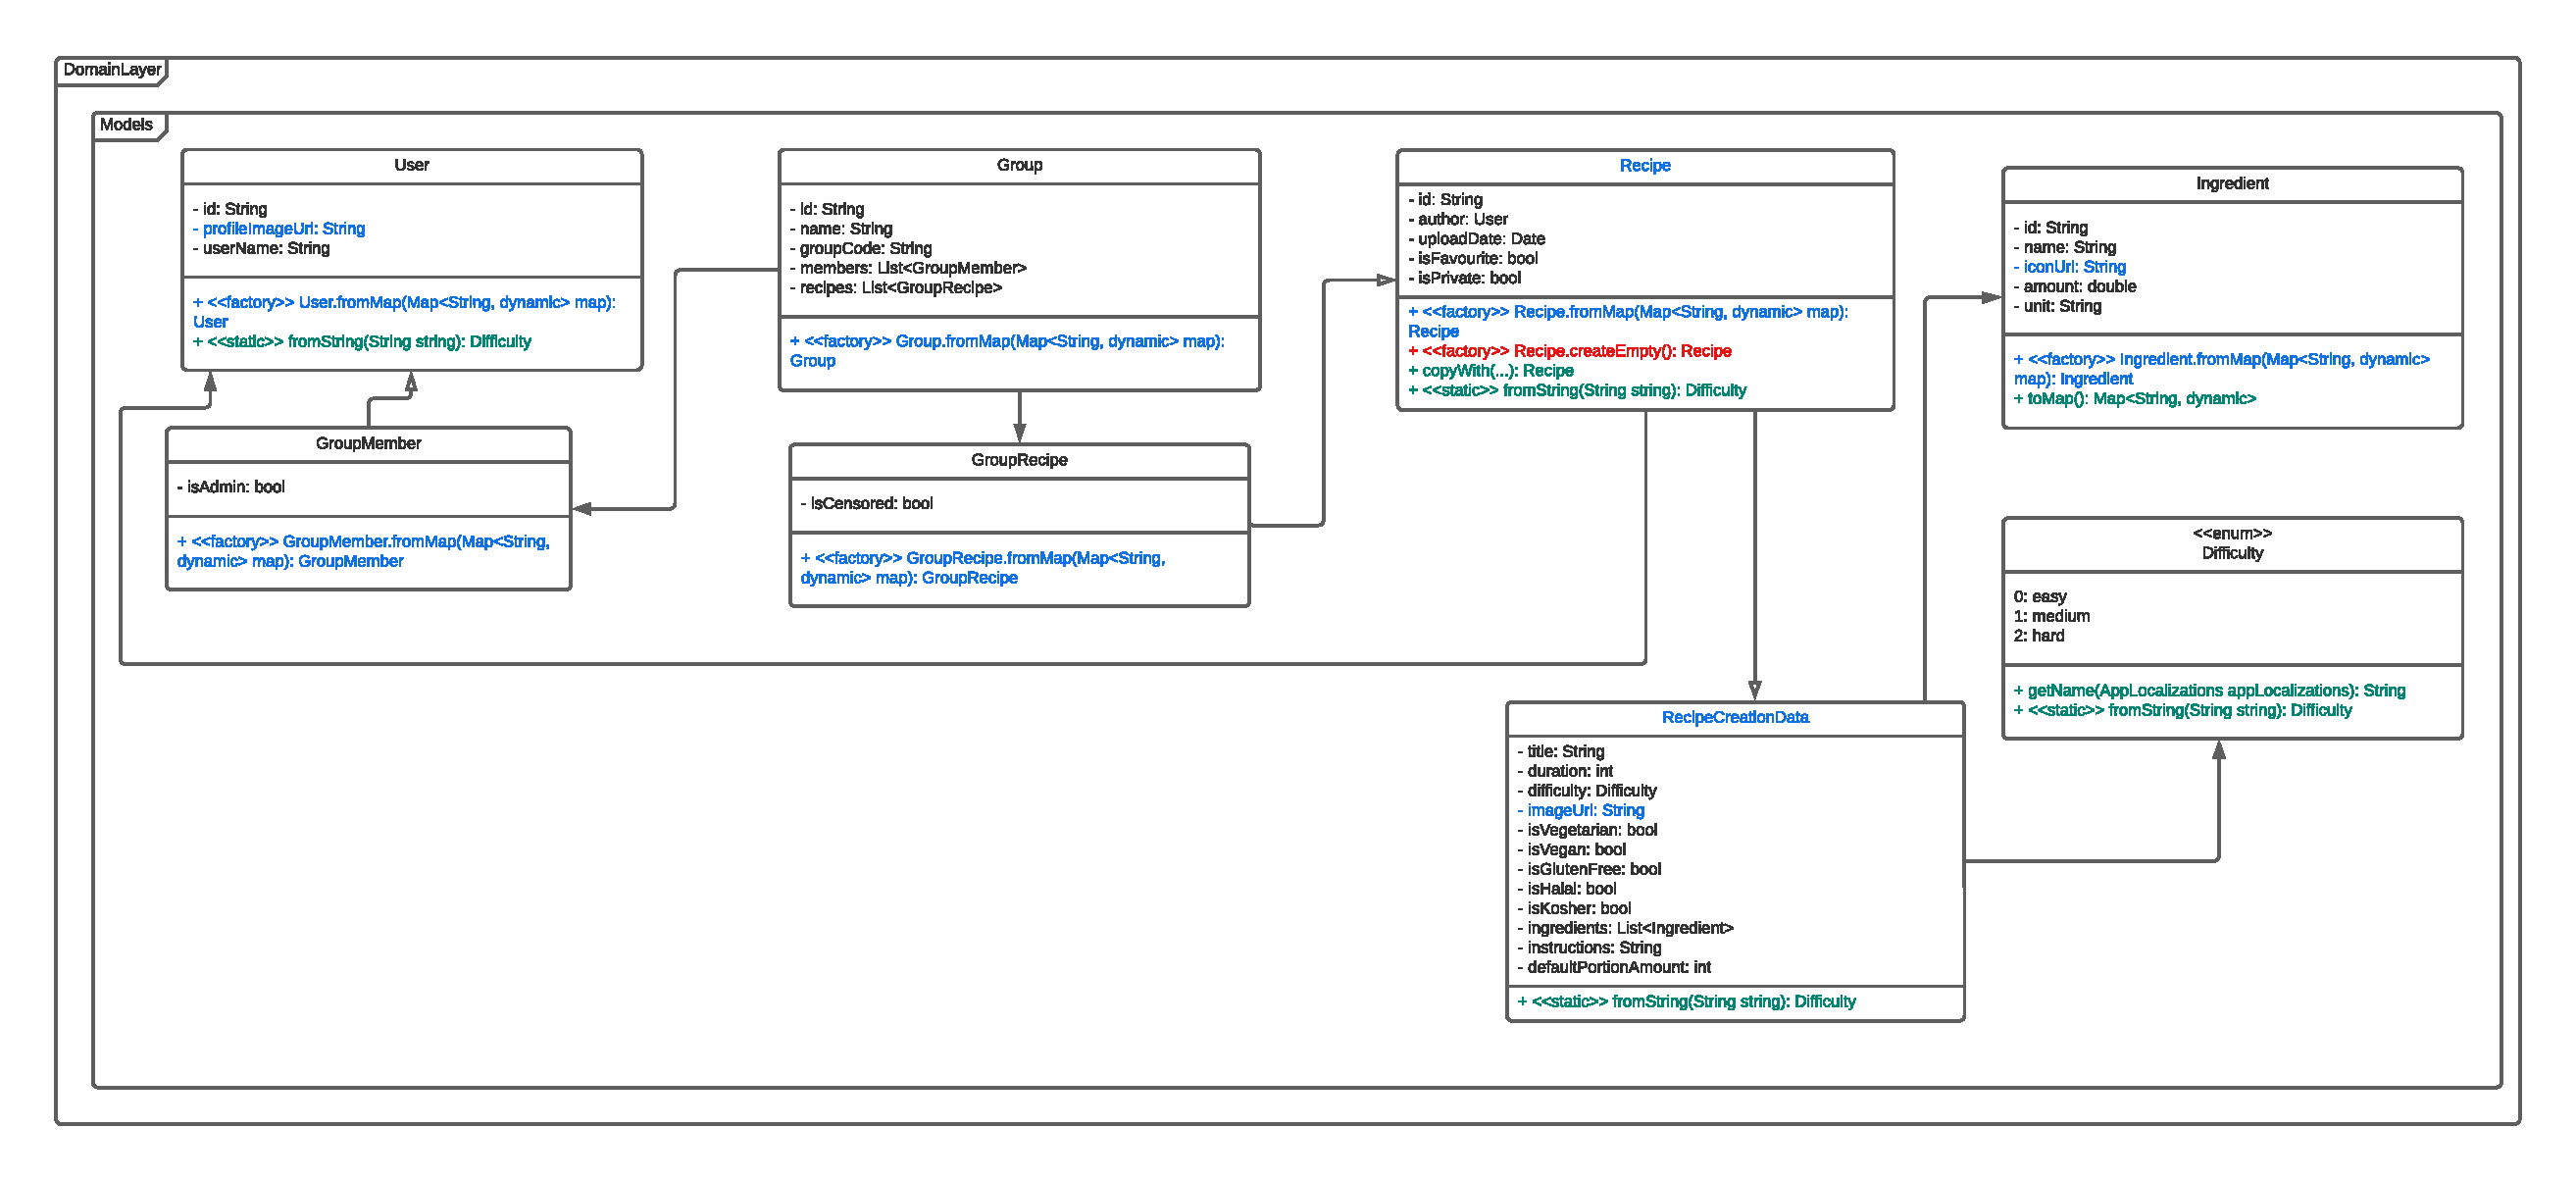
\includegraphics[width=0.95\textwidth]{images/uml/modellayer.pdf}
    \caption{Änderungen am Modellayer}
    \label{fig:modellayer}
\end{figure}
\paragraph*{\texttt{fromMap(Map<String, dynamic> map)}} Die Factory-Methoden \texttt{fromJson} wurden in \texttt{fromMap} umbenannt, da sie unabhängig von der Serialisierungsmethode sind.
\paragraph*{\texttt{toMap()}} Die statische Methode \texttt{toMap} wurde bei einigen Klassen hinzugefügt, um die Serialisierung zu vereinfachen. Sie gibt ein \texttt{Map<String, dynamic>} zurück, das die Attribute der Klasse enthält.
\paragraph{\texttt{Recipe} und \texttt{RecipeCreationData}}
Die Klasse \texttt{Recipe} wurde in die beiden Klassen \texttt{Recipe} und \texttt{RecipeCreationData} aufgeteilt. Die Klasse \texttt{Recipe} enthält nur noch die Attribute, die ein Rezept nach der Erstellung haben kann, wie zum Beispiel den Author und die Id. Die Klasse erbt von \texttt{RecipeCreationData}, die die Attribute enthält, die ein Rezept bei der Erstellung haben muss, wie Namen oder Anweisungen.
\paragraph{\texttt{Recipe.copyWith(...)}} Die Methode \texttt{copyWith} wurde hinzugefügt, um ein Rezept zu kopieren und dabei einzelne Attribute zu ändern. Die zuändernden Attribute werden als benannte Parameter übergeben.
\paragraph{\texttt{Recipe.createEmpty()}} Die Methode wurde entfernt, da sie nicht mehr benötigt wird.
\paragraph{\texttt{Difficulty.getName(BuildContext context): String}}
Die Methode gibt einen String zurück, der den Namen der Schwierigkeit in der aktuellen Sprache enthält. Die Sprache wird aus dem \texttt{BuildContext} gelesen.
\paragraph{\texttt{Difficulty.fromString(String string)}}
Die statische Methode gibt die Schwierigkeit zurück, die den übergebenen String als Namen hat.
\paragraph{\texttt{RecipeCreationData.imageUrl} und \texttt{Ingredient.iconUrl}} Wir haben uns dazu entschieden statt dem Icon/Bild selbst nur die URL zu speichern. Damit können wir die Anfragengröße massiv verkleinern. Mehr dazu folgt im Kapitel \ref{sec:images}.
\subsection{Änderungen am Datalayer}

\subsection{Hinzufügen eines ORM (Object-Relational Mapping) im Backend}
Anstatt wie im ursprünglichen Entwurf die Datenbankzugriffe direkt über die Klasse \texttt{Database} zu machen, haben wir uns dazu entschieden ein ORM zu verwenden.
Wir haben uns für das ORM \texttt{Prisma} entschieden, da es uns die Möglichkeit gibt, die Datenbank in einer \texttt{.prisma}-Datei zu definieren und dann automatisch die Datenbankzugriffe zu generieren.

Prisma bietet eine leistungsfähige und intuitive Möglichkeit, Datenmodelle zu definieren. Die Unterstützung von Prisma für relationale Datenbanken wie PostgreSQL, MySQL und SQLite ermöglicht uns eine nahtlose Integration mit unseren vorhandenen Datenbanken. Durch die Verwendung einer dedizierten Schema-Sprache können wir Datenmodelle klar und präzise darstellen, was die Zusammenarbeit im Team erleichtert und die Fehleranfälligkeit verringert.
Prisma bietet zudem integrierte Funktionen zum Schutz vor SQL-Injections und anderen Sicherheitsbedrohungen. Indem es Parameterized Queries verwendet, minimiert Prisma das Risiko von Angriffen auf unsere Datenbanken. Diese Sicherheitsfunktionen sind für unsere Anwendung von entscheidender Bedeutung, da wir sensible Benutzerdaten verarbeiten.
Dank des leistungsstarken Query Builders von Prisma können wir komplexe Datenbankabfragen effizient und ressourcenschonend erstellen. Prisma generiert optimierten SQL-Code, der die Datenbanklast minimiert und gleichzeitig eine hohe Performance gewährleistet. Dies ist besonders wichtig, da unsere Anwendung mit zunehmender Benutzerzahl und Datenmenge skaliert.
Die Entscheidung, Prisma als ORM in unserer Anwendung einzusetzen, hat sich als äußerst vorteilhaft erwiesen. Die leistungsfähige Datenmodellierung, Sicherheitsfunktionen, Performance-Optimierungen und die Unterstützung für verschiedene Datenbanken bieten uns eine robuste und skalierbare Grundlage für unsere Entwicklungsstrategie. Prisma ermöglicht es uns, uns auf die Entwicklung von Funktionen und die Verbesserung der Benutzererfahrung zu konzentrieren, während es gleichzeitig die Datenbankverwaltung und Abfragen effizient bewältigt.


\subsection{Änderungen an der Server- und Applicationklasse}

\begin{figure}[htp]
    \centering
    \includegraphics[width=0.95\textwidth]{example-image-a}
    \caption{Änderungen an der Server- und Applicationklasse}
    \label{fig:server}
\end{figure}
\paragraph{\texttt{connectToDatabase()}} Die Methode wurde entfernt, da sie nicht mehr benötigt wird.

\paragraph{\texttt{imageRouter: ImageRouter}} Die Attribute wurde hinzugefügt um die ImageRouter-Klasse zu initialisieren.

\subsection{Änderungen an den Routern}
\begin{figure}[htp]
    \centering
    \includegraphics[width=0.95\textwidth]{example-image-a}
    \caption{Änderungen an den Routern}
    \label{fig:routers}
\end{figure}

Es wurden sowohl bei dem \texttt{GroupRouter} als auch beim \texttt{AdminUserRouter} folgende Attribute hinzugefügt.

\paragraph{\texttt{checkGroupMemberState: CheckGroupMemberState}} Die Attribute wurde hinzugefügt um die CheckGroupMemberState-Klasse zu initialisieren.
\paragraph{\texttt{checkMemberStateTarget: any}} 

\subsection{Änderungen an den Controllern}

Bei allen Controllerfunktionen wurde das Request-Argument typsicher gemacht, d.h. es ist klar definiert, welche Argumente in head und body übergeben werden. 
Außerdem werden eventuell auftretende Fehler mit der next function an den Errorhandler weitergegeben. Die Klasse \texttt{ImageController} wurde hinzugefügt, um Bilder zu verwalten. 
\texttt{RecipeController} und \texttt{UserController} halten eine Instanz von \texttt{Imagecontroller}

\paragraph{\texttt{AbstractController}} Die Attribute \texttt{pool} und \texttt{database} wurden entfernt. Datenbankanfragen werden nun mithilfe des PrismaClients über das Attribut \texttt{prisma} ausgeführt. 
Außerdem wurden die Attribute \texttt{firebaseAuth} und \texttt{firebaseAdmin} hinzugefügt, um die Authentifizierung mit Firebase zu ermöglichen.

\paragraph{\texttt{UserController}} Die Methode getUser wurde hinzugefügt, um einen Benutzer anhand seines idTokens zu erhalten.

\paragraph{\texttt{AuthentificationController}} Die Methode \texttt{userGetByIdToken} wurde entfernt und durch die Methode \texttt{getUser} im UserController ersetzt.

\paragraph{\texttt{IngredientController}} Die Methode \texttt{ingredientIconGet} wurde hinzugefügt, um alle Icons als URL zu erhalten. Die Methode \texttt{ingredientIconGetById} wurde hinzugefügt, um ein Icon anhand seiner ID als Bytearray zu erhalten.

\subsection{Änderungen an der Middleware} Wie auch bei den Controllern, wurden auch bei der Middleware alle Request-Argumente typsicher gemacht. Die Klassen \texttt{AbstractMiddle}, \texttt{CheckGroupMemberState}, \texttt{SchemaValidator} und \texttt{AuthenticatedRequest} wurden neu hinzugefügt.

\paragraph{\texttt{AbstractMiddleware}} Klasse, von der alle anderen Middlewareklassen erben. Sie enthält einen Constructor und das Attribut \texttt{prisma : PrismaClient} um Datenbankanfragen auszuführen.

\paragraph{\texttt{AuthenticatedRequest}} Interface, das texttt{express.Request} um das Atrribut \texttt{userId : string} erweitert.

\paragraph{\texttt{CheckGroupMemberState}} Klasse, die überprüft, ob ein Benutzer Mitglied einer Gruppe ist. Dazu wird die Methode \texttt{checkMemberStateTarget(express.Request, express.Response, express.NextFunction)} verwendet.

\paragraph{\texttt{SchemaValidator}} Klasse, die die Requestdaten anhand eines Joi-Schemas validiert. Dazu wird die Methode \texttt{validateRequest(schema: joi.objectSchema)} verwendet.

\paragraph{\texttt{CheckAuthorization}} Die Methode \texttt{checkAuthorization} findet nun zusätzlich den Nutzer in der Datenbank und fügt seine Id der Request hinzu. Weitergegeben wird eine \texttt{AuthenticatedRequest}.

\section{Validierung von Eingaben}
Bei der Entwicklung von TypeScript-Anwendungen ist die Dateneingabevalidierung von entscheidender Bedeutung, um die Integrität und Sicherheit unserer Anwendung zu gewährleisten. Die Bibliothek Joi hat sich als eine der beliebtesten und effektivsten Lösungen für die Validierung von Daten in JavaScript erwiesen. Wir haben uns deshalb für diese leistungsstarke Validierungs-Bibliothek entschieden haben.
Alle Request, die gestellt werden können werden dabei mit Joi validiert. Dabei wird überprüft, ob alle benötigten Felder vorhanden sind und ob die Felder den richtigen Datentyp haben.

Dafür hat jeder Controller ein Joi-Schema, das die Validierung beschreibt. Dieses Schema wird dann in der \texttt{validateRequest}-Middleware verwendet, um die Request zu validieren.

In der Abbildung \ref{fig:validation} sind die Schemas als UML-Diagramm dargestellt.



\section{Grafische Benutzeroberfläche}
Das Design der grafischen Benutzeroberfläche änderte sich nicht wesentlich von dem, was wir uns im Pflichtenheft überlegt hatten.
Es kam nur zu kleinen Änderungen, wie sie im Kapitel \ref{sec:changes} beschrieben sind.
\newpage
\section{Glossar}
\printglossary[style=altlist]
\end{document}